%% !TEX program = xelatex
%% -----------------------------------------------------------------
%% This file uses UTF-8 encoding
%%
%% For compilation use following command:
%% $ latexmk -pdf -pvc thesis
%%
%% -----------------------------------------------------------------
%%                                     _     _
%%      _ __  _ __ ___  __ _ _ __ ___ | |__ | | ___
%%     | '_ \| '__/ _ \/ _` | '_ ` _ \| '_ \| |/ _ \
%%     | |_) | | |  __/ (_| | | | | | | |_) | |  __/
%%     | .__/|_|  \___|\__,_|_| |_| |_|_.__/|_|\___|
%%     |_|
%%
%% -----------------------------------------------------------------

\documentclass[
    mainlanguage=slovak,    % Main language of the thesis
    otherlanguage=english   % Other language of the thesis
]{tukethesis}

% Additional packages
% \usepackage{algorithm}

% !TEX root = thesis.tex

%% Document Metadata

\title{SalonCRM -- CRM System for a Beauty Salon}{SalonCRM -- CRM systém pre kozmetický salón}
\thesis{Semester project}{Semestrálny projekt}

%% The class supports only one author; it is used for PDF metadata only.
%% The title page prints \projectauthors (see thesis.tex).
\author[Bc.]{Martin}{Saxa}
\newcommand{\projectauthors}{%
  Bc.~Martin Saxa \\
  Bc.~Jakub Spišák \\
  Bc.~Roman Šafranko \\
  Bc.~Samuel Šarkan%
}

\submissiondate{4}{11}{2026}

%% Required by the class for PDF metadata, not printed.
\keywords{}{}
                    % Load thesis metadata

\emergencystretch=3em  % fewer overfull lines with long \texttt

% Title page for a project with multiple authors
\makeatletter
\newcommand{\projecttitlepage}{
    \begin{center}
        {\Large \textbf{\@college}}

        {\Large \textbf{\@faculty}}

        \vfill

        {\LARGE \textbf{\@title} \par}

        \bigskip

        {\large \textbf{\@thesis}}
    \end{center}

    \vfill

    \noindent
    {\Large \textbf{\@college@city{} \@submissionyear}} \hfill
    {\large \textbf{\begin{tabular}[b]{@{}r@{}}\projectauthors\end{tabular}}}

    \newpage
}
\AtBeginDocument{\hypersetup{pdfauthor={Martin Saxa, Jakub Spišák, Roman Šafranko, Samuel Šarkan}}}
\makeatother


%% -----------------------------------------------------------------
%%          _                                       _
%%       __| | ___   ___ _   _ _ __ ___   ___ _ __ | |_
%%      / _` |/ _ \ / __| | | | '_ ` _ \ / _ \ '_ \| __|
%%     | (_| | (_) | (__| |_| | | | | | |  __/ | | | |_
%%      \__,_|\___/ \___|\__,_|_| |_| |_|\___|_| |_|\__|
%%
%% -----------------------------------------------------------------

\begin{document}

%% Title page and table of contents
\pagenumbering{roman}
\pagestyle{empty}
\projecttitlepage

\pagestyle{plain}
\tableofcontents
\newpage

\pagestyle{fancy}
\pagenumbering{arabic}

%% List of chapters in required order
% !TEX root = ../thesis.tex

\chapter{Zadanie a analýza}\label{ch:analysis}

\section{Zadanie}

Cieľom projektu je vytvoriť vnútropodnikový informačný systém pre kozmetický salón. Systém má podobu CRM (\emph{Customer Relationship Management}) a slúži na správu zákazníkov, objednávok (termínov) a platieb. Okrem bežnej evidencie má salónu pomôcť udržať si zákazníkov: pomocou strojového učenia predikuje, ktorí zákazníci pravdepodobne prestanú chodiť, aby ich mohol personál včas osloviť.

Zo zadania predmetu vyplývajú tieto technické požiadavky:

\begin{itemize}
  \item podnikový informačný systém postavený na prepojených aplikačných webových službách,
  \item prihlasovanie a odhlasovanie, aspoň dve používateľské roly a práca so sessions,
  \item hlavný backend, ktorý obsluhuje aspoň dve obrazovky,
  \item druhý backend v inom programovacom jazyku (nemusí mať vlastné používateľské rozhranie),
  \item frontend, ktorý spája dáta z oboch backendov,
  \item dve samostatné SQL databázy,
  \item komponent strojového učenia,
  \item procesný model v notácii BPMN,
  \item nasadenie pomocou kontajnerov.
\end{itemize}

\section{Rozdelenie úloh v tíme}

Projekt riešil štvorčlenný tím. Rozdelenie rolí uvádza tabuľka~\ref{tab:team}.

\begin{table}[ht]
  \centering
  \caption{Roly členov tímu}\label{tab:team}
  \begin{tabular}{@{}llp{.45\textwidth}@{}}
    \toprule
    Rola & Člen tímu & Zodpovednosť \\
    \midrule
    AI expert & Roman Šafranko & ML služba, príznaky, tréning a vyhodnotenie modelu \\
    Doménový expert & Martin Saxa & požiadavky salónu, analýza domény, procesy (BPMN) \\
    Softvérový architekt & Samuel Šarkan & architektúra, rozhrania služieb, nasadenie \\
    Softvérový inžinier & Jakub Spišák & implementácia backendu a frontendu \\
    \bottomrule
  \end{tabular}
\end{table}

\section{Analýza domény}

Kozmetický salón ponúka služby rozdelené do kategórií (ošetrenie pleti, nechty, obočie a mihalnice, depilácia, masáže, líčenie). Každá služba má dĺžku trvania a cenu a vykonávajú ju iba niektorí pracovníci. Salón má pevné otváracie hodiny a termíny sa plánujú v 15-minútovej mriežke.

V systéme vystupujú tri skupiny používateľov:

\begin{description}
  \item[Zákazník] nemá účet. Rezervuje si termín cez verejný formulár: vyberie službu, pracovníka (alebo „ktokoľvek“), voľný čas a zadá kontaktné údaje. Identifikuje sa e-mailom; ak zákazník s rovnakým e-mailom už existuje, termín sa priradí k nemu.
  \item[Pracovník (rola \texttt{User})] napríklad kozmetička. Vidí svoj kalendár, spravuje iba svoje termíny a iba zákazníkov, ktorých obsluhoval. Termín môže dokončiť (a zaevidovať platbu), zrušiť, označiť ako nedostavenie sa alebo preplánovať. Telefonické objednávky zapisuje za zákazníka.
  \item[Administrátor (rola \texttt{Admin})] vidí všetky dáta, spravuje používateľov, služby a cenník, sleduje štatistiky (tržby, návštevy, vyťaženosť pracovníkov) a pracuje s výsledkami predikcie odchodu zákazníkov.
\end{description}

Životný cyklus termínu je jednoduchý stavový automat. Nový termín je v stave \emph{naplánovaný}. Odtiaľ môže prejsť do stavu \emph{dokončený} (spolu so zápisom platby), \emph{zrušený} alebo \emph{neprišiel}. Všetky tri sú konečné. Dôležitým obchodným pravidlom je, že pracovník nesmie mať dva prekrývajúce sa termíny. Kontrola iba v aplikácii nestačí, pretože dvaja zákazníci môžu ten istý čas rezervovať súčasne. Preto prekrývaniu bráni aj obmedzenie priamo v databáze.

\section{Predikcia odchodu zákazníka}

Pre salón je lacnejšie udržať si existujúceho zákazníka ako získať nového. Systém preto pre každého zákazníka s aspoň dvoma dokončenými návštevami odhaduje pravdepodobnosť, že v nasledujúcich 90 dňoch nepríde (tzv. \emph{churn}). Výsledok má podobu pravdepodobnosti, úrovne rizika (nízke, stredné, vysoké) a čitateľného zdôvodnenia, napríklad: „Posledná návšteva pred 64 dňami, obvykle chodí každých 21 dní. Nemá naplánovaný ďalší termín.“

Model sa učí z histórie termínov. Príznaky opisujú správanie zákazníka k zvolenému dátumu: počet dní od poslednej návštevy, priemerný interval medzi návštevami a ich pomer, počet návštev za posledných 90 a 180 dní, útrata, podiel zrušených termínov, existencia budúceho termínu a najčastejšia kategória služby. Pri ich výpočte sa používajú iba údaje, ktoré boli k danému dátumu známe, aby model „nevidel do budúcnosti“ (\emph{data leakage}).

Trénuje sa niekoľko klasifikátorov z knižnice scikit-learn (logistická regresia, náhodný les a gradient boosting). Vyhodnocujú sa na časovo oddelenej validačnej množine a porovnávajú s jednoduchým pravidlom (zákazník nechodí viac ako dvojnásobok svojho obvyklého intervalu). Vyberie sa model s najvyššou hodnotou ROC-AUC. Na základe predikcie môže administrátor zaznamenať \emph{retenčnú akciu}, teda kontakt so zákazníkom telefonicky, e-mailom alebo osobne.

Keďže salón nemá reálne historické dáta, systém pracuje so syntetickými dátami. Tie modelujú rôzne typy zákazníkov (verní, nepravidelní, odchádzajúci, jednorazoví) aj so zámerným šumom. Dosiahnuté metriky preto preukazujú funkčnosť celého postupu, nie presnosť na reálnych dátach.

% !TEX root = ../thesis.tex

\chapter{Architektúra}\label{ch:architecture}

Systém tvoria štyri hlavné časti: webový frontend, hlavný backend, ML backend a dve databázy. Ich prepojenie zobrazuje obrázok~\ref{fig:architecture}.

\begin{figure}[ht]
  \centering
  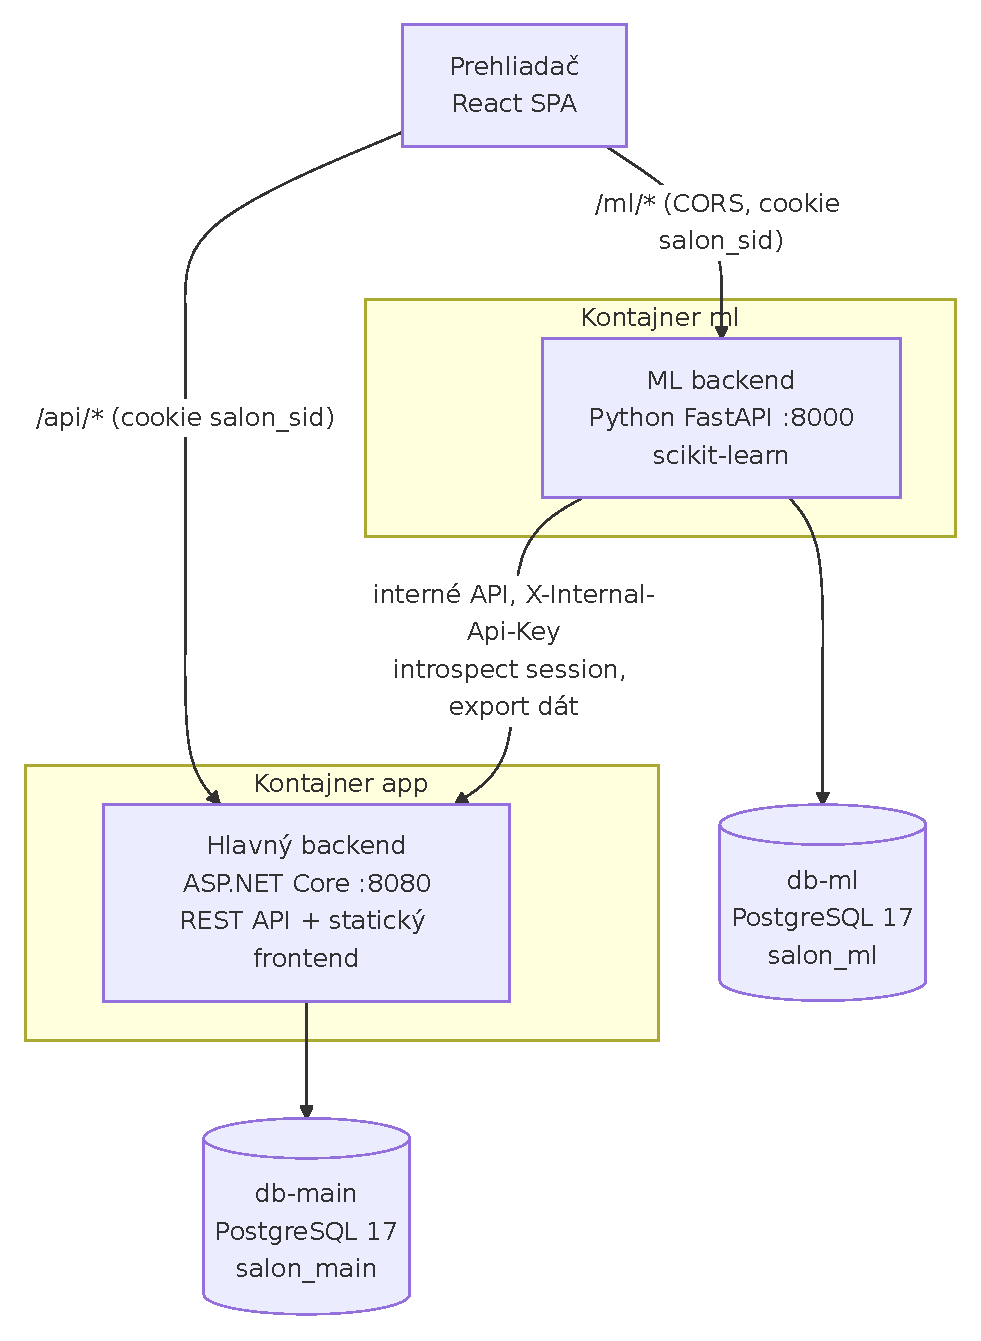
\includegraphics[width=.8\textwidth]{figures/architecture.pdf}
  \caption{Architektúra systému SalonCRM}\label{fig:architecture}
\end{figure}

\section{Komponenty}

\paragraph{Frontend} je jednostránková aplikácia (SPA) napísaná v jazyku TypeScript s knižnicou React a nástrojom Vite. Na načítanie dát používa TanStack Query, formuláre validuje knižnicou zod, kalendár termínov zobrazuje cez FullCalendar a grafy cez Recharts. Obsahuje dvoch API klientov: jeden pre hlavný backend (\texttt{/api/*}) a druhý pre ML backend (\texttt{/ml/*}). Viaceré obrazovky kombinujú dáta z oboch. Napríklad kalendár a zoznam zákazníkov dopĺňajú k zákazníkom farebný odznak rizika odchodu a ML dashboard dopĺňa k predikciám mená zákazníkov z hlavného backendu.

\paragraph{Hlavný backend} je REST API v ASP.NET Core (.NET 10) s prístupom do databázy cez Entity Framework Core. Je usporiadaný do vertikálnych rezov podľa oblastí (autentifikácia, verejná rezervácia, termíny, zákazníci, používatelia, služby, štatistiky). Obsluhuje všetky obrazovky okrem ML dashboardu a v produkcii servíruje aj zostavený frontend.

\paragraph{ML backend} je REST API v jazyku Python s frameworkom FastAPI. Nemá vlastné používateľské rozhranie. Na prácu s dátami používa pandas, na strojové učenie scikit-learn a natrénované modely ukladá cez joblib. Zabezpečuje synchronizáciu dát, tréning, predikciu a sprístupnenie výsledkov.

\paragraph{Databázy.} Každý backend má vlastnú inštanciu PostgreSQL 17. Databáza \texttt{salon\_main} obsahuje používateľov, sessions, služby, zákazníkov, termíny, platby a retenčné akcie. Databáza \texttt{salon\_ml} obsahuje kópiu pseudonymizovaných dát na tréning, verzie modelov s metrikami a históriu predikcií. Žiadny backend nečíta databázu toho druhého. Jediným prepojením je HTTP komunikácia.

\section{Komunikácia medzi službami}

Frontend komunikuje s oboma backendmi priamo. ML backend volá interné API hlavného backendu, ktoré je chránené zdieľaným kľúčom v hlavičke \texttt{X-Internal-Api-Key}. Interné API má dva endpointy:

\begin{itemize}
  \item \nolinkurl{POST /api/internal/sessions/introspect} overí session prihláseného používateľa a vráti jeho rolu,
  \item \nolinkurl{GET /api/internal/ml/export} vráti zákazníkov a termíny na tréning modelu.
\end{itemize}

Export obsahuje iba pseudonymné identifikátory a údaje o termínoch (čas, stav, kategória služby, cena). Mená, e-maily, telefóny a poznámky do ML služby neprechádzajú, čím sa dodržiava princíp minimalizácie dát.

\section{Autentifikácia a sessions}

Prihlásenie zabezpečuje hlavný backend. Po overení hesla vygeneruje náhodný token, ktorý odošle prehliadaču v cookie \texttt{salon\_sid} s príznakmi \texttt{HttpOnly} a \texttt{SameSite=Lax}. V tabuľke \texttt{sessions} sa uloží iba hash tokenu. Session platí najviac 12 hodín a po dvoch hodinách nečinnosti vyprší. Odhlásenie session zneplatní a administrátor vidí zoznam aktívnych sessions a môže ich rušiť.

ML backend vlastné prihlasovanie nemá. Pri chránenom požiadavku prečíta tú istú cookie a overí ju cez introspekciu v hlavnom backende. Výsledok si na krátky čas uloží do cache. Cookie sa na ML backend dostane vďaka tomu, že oba backendy patria k rovnakému webu (\emph{site}): lokálne aj v produkcii na Azure bežia na rovnakom hostiteľovi, iba s iným portom. ML backend povoľuje CORS s prihlasovacími údajmi iba pre konkrétne originy.

Autorizácia je explicitná na každom endpointe. Obmedzenie pracovníka iba na jeho vlastné termíny a zákazníkov je súčasťou databázového dotazu, nie iba používateľského rozhrania. Záznam, ktorý pracovníkovi nepatrí, sa správa, akoby neexistoval (HTTP 404).

\section{ML pipeline}

Administrátor spúšťa pipeline tlačidlom „Prepočítať predikcie“ v ML dashboarde. Beh má tieto kroky:

\begin{enumerate}
  \item stiahnutie exportu z hlavného backendu a jeho uloženie do \texttt{salon\_ml},
  \item vytvorenie trénovacích príkladov z historických snapshotov (vždy s celým 90-dňovým horizontom v minulosti, aby bol známy skutočný výsledok),
  \item tréning kandidátov a ich vyhodnotenie na najnovšom snapshote voči jednoduchému pravidlu,
  \item výber najlepšieho modelu, výpočet dôležitosti príznakov, pretrénovanie na všetkých dátach a uloženie novej verzie modelu,
  \item predikcia pre všetkých zákazníkov s dostatočnou históriou a uloženie výsledkov s vysvetlením.
\end{enumerate}

Predikcie sa nemažú, takže je možné sledovať vývoj rizika konkrétneho zákazníka v čase.

% !TEX root = ../thesis.tex

\chapter{Nasadenie}\label{ch:deployment}

\section{Kontajnery}

Celý systém je zabalený do kontajnerov. Na lokálny vývoj a demonštráciu sa spúšťa pomocou Docker Compose. Základ tvoria štyri kontajnery (tabuľka~\ref{tab:containers}).

\begin{table}[ht]
  \centering
  \caption{Kontajnery systému}\label{tab:containers}
  \begin{tabular}{@{}llp{.5\textwidth}@{}}
    \toprule
    Kontajner & Port & Obsah \\
    \midrule
    \texttt{db-main} & 5432 & PostgreSQL 17, databáza \texttt{salon\_main} \\
    \texttt{db-ml}   & 5433 & PostgreSQL 17, databáza \texttt{salon\_ml} \\
    \texttt{app}     & 8080 & ASP.NET Core API spolu so zostaveným frontendom \\
    \texttt{ml}      & 8000 & FastAPI a ML pipeline \\
    \bottomrule
  \end{tabular}
\end{table}

Obraz \texttt{app} sa zostavuje viacstupňovo: najprv sa v Node.js zostaví frontend, potom sa v .NET SDK skompiluje backend a nakoniec sa oba výstupy skopírujú do runtime obrazu ASP.NET Core. Hlavný backend tak servíruje statické súbory frontendu a všetky cesty mimo \texttt{/api} presmeruje na \texttt{index.html}, kým neznáma API cesta vráti chybu 404 vo formáte JSON. Pri štarte kontajnera sa automaticky aplikujú databázové migrácie a naplnia sa ukážkové dáta. Kontajner \texttt{ml} pri štarte aplikuje migrácie nástrojom Alembic a spustí server uvicorn.

Databázy majú zdravotné kontroly (\texttt{pg\_isready}) a backendy štartujú až po tom, čo je ich databáza pripravená. Dáta oboch databáz a natrénované modely sú uložené v pomenovaných zväzkoch, takže prežijú reštart aj výmenu kontajnerov. Konfigurácia a tajomstvá (heslá databáz, interný API kľúč, povolené originy pre CORS, adresa ML služby) sa odovzdávajú výhradne cez premenné prostredia zo súboru \texttt{.env}.

Lokálne sa celý systém spustí príkazom \texttt{docker compose up -{}-build} a je dostupný na adrese \url{http://localhost:8080}.

\section{Nasadenie na Azure}

V produkcii sa namiesto Docker Compose použijú spravované služby platformy Microsoft Azure (obrázok~\ref{fig:deployment}). Oba backendy bežia ako kontajnery v službe Azure App Service (Web App for Containers) a databázy poskytuje služba Azure Database for PostgreSQL. Azure sa tak stará o prevádzku servera, aktualizácie, HTTPS certifikáty aj zálohovanie databáz.

\begin{figure}[ht]
  \centering
  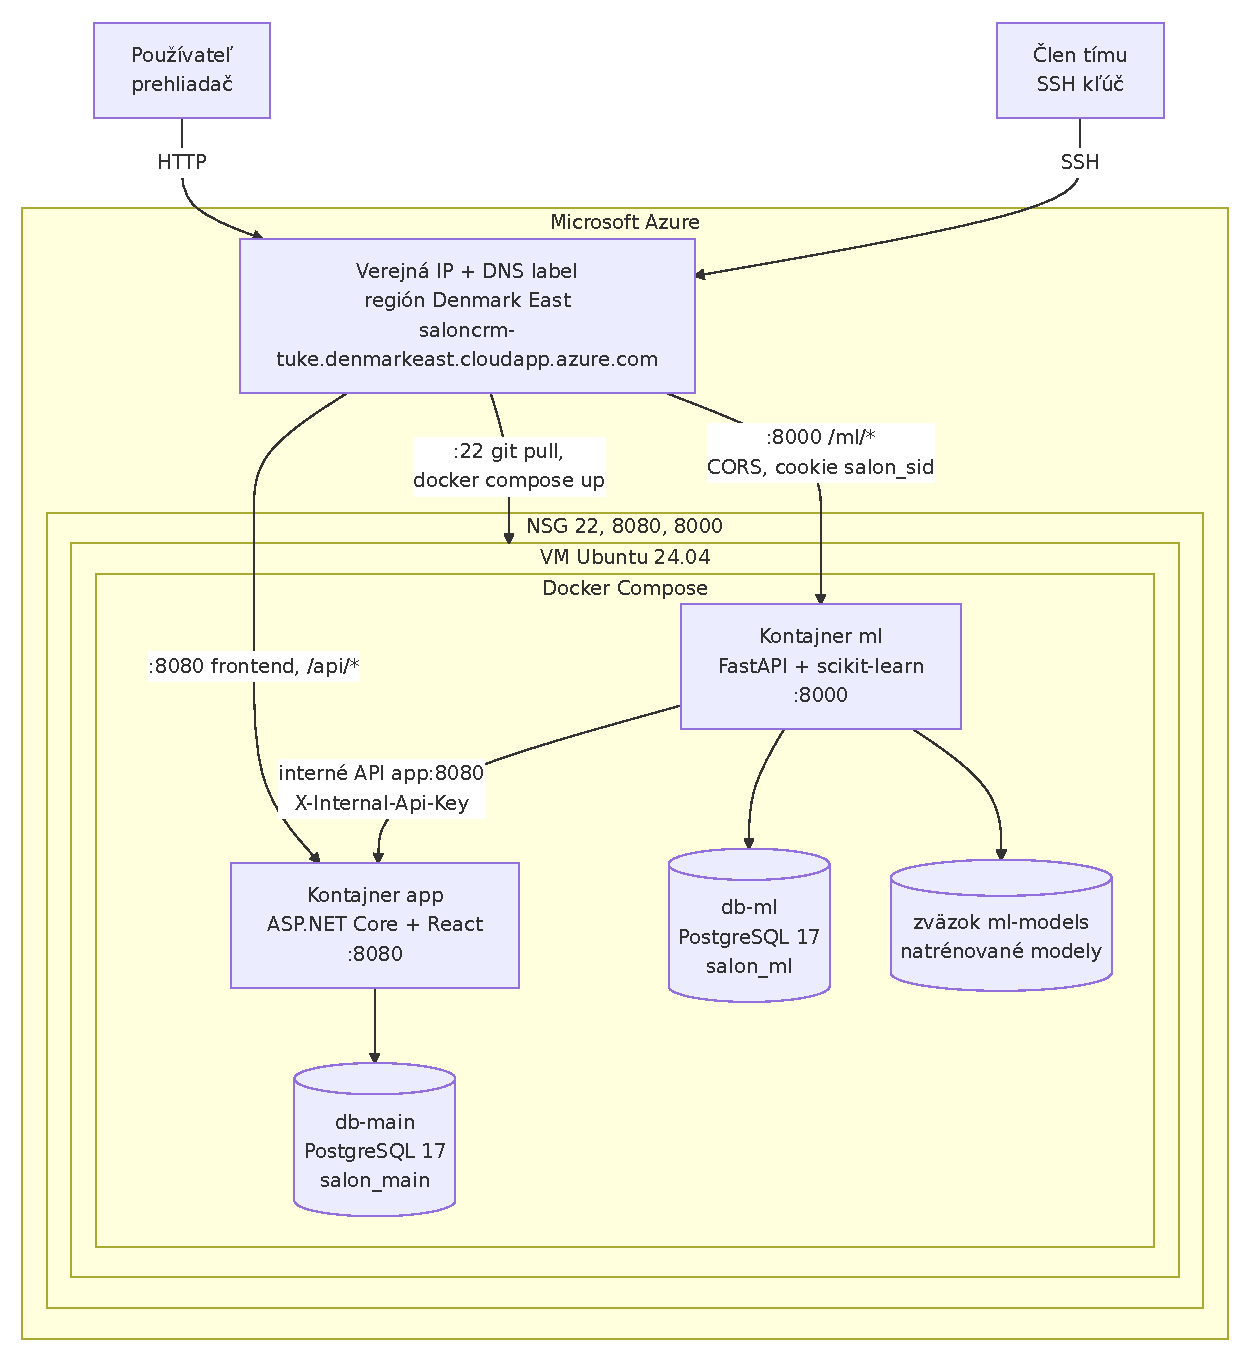
\includegraphics[width=\textwidth]{figures/deployment.pdf}
  \caption{Nasadenie v Azure}\label{fig:deployment}
\end{figure}

\subsection*{Aplikácie}

V jednom App Service pláne s Linuxom bežia dve webové aplikácie. Každá spúšťa ten istý Docker obraz, ktorý sa používa lokálne:

\begin{description}
  \item[Web App \texttt{app}] hlavný backend spolu so zostaveným frontendom,
  \item[Web App \texttt{ml}] ML backend.
\end{description}

App Service zabezpečuje HTTPS, preto sa cookie \texttt{salon\_sid} posiela s príznakom \texttt{Secure}. Obe aplikácie dostanú vlastnú doménu ako subdomény jednej registrovanej domény (napr. \nolinkurl{salon.<doména>} a \nolinkurl{ml.<doména>}). Predvolené adresy \nolinkurl{*.azurewebsites.net} sa nepoužívajú, pretože prehliadač ich považuje za rôzne weby (\emph{sites}). Cookie so \texttt{SameSite=Lax} by sa potom na ML backend neposlala. Pod spoločnou doménou sa cookie posiela obom backendom rovnako ako pri lokálnom vývoji.

ML backend volá interné API hlavného backendu cez jeho HTTPS adresu, chránené kľúčom v hlavičke \texttt{X-Internal-Api-Key}. Natrénované modely sa ukladajú do trvalého úložiska App Service (adresár \texttt{/home}, premenná \texttt{MODEL\_DIR}), takže prežijú reštart aj nasadenie novej verzie.

\subsection*{Databázy}

Kontajnery \texttt{db-main} a \texttt{db-ml} v produkcii nahrádza Azure Database for PostgreSQL -- Flexible Server s verziou PostgreSQL 17. Na serveri sú dve samostatné databázy, \texttt{salon\_main} a \texttt{salon\_ml}. Každý backend má vlastného databázového používateľa s právami iba na svoju databázu, takže oddelenie dát zostáva zachované. Spojenie je šifrované (TLS) a firewall servera povoľuje prístup iba zo služieb Azure. Rozšírenie \texttt{btree\_gist}, ktoré potrebuje obmedzenie proti prekrývaniu termínov, treba na serveri povoliť v parametri \texttt{azure.extensions}.

\subsection*{Konfigurácia a postup nasadenia}

Konfigurácia sa nastavuje v \emph{Application settings} webových aplikácií. Tie App Service odovzdá kontajneru ako premenné prostredia, rovnako ako súbor \texttt{.env} lokálne. Ide najmä o reťazce pripojenia k databázam, interný API kľúč, adresu hlavného backendu pre ML službu, povolené originy CORS a príznak \texttt{Secure} pre cookie. Adresa ML služby sa zapisuje do frontendu pri zostavení obrazu, preto sa obraz \texttt{app} zostavuje už s produkčnou adresou.

Postup nasadenia:

\begin{enumerate}
  \item vytvorenie skupiny prostriedkov, PostgreSQL servera s dvoma databázami a dvoma používateľmi a povolenie rozšírenia \texttt{btree\_gist},
  \item vytvorenie App Service plánu a dvoch webových aplikácií pre kontajnery,
  \item nastavenie vlastnej domény a certifikátov pre obe aplikácie,
  \item nastavenie \emph{Application settings} (tajomstvá iba tu, nie v repozitári),
  \item zostavenie Docker obrazov v GitHub Actions a ich nahratie do registra kontajnerov,
  \item nasadenie obrazov do webových aplikácií; migrácie databáz sa aplikujú automaticky pri štarte kontajnerov.
\end{enumerate}

Kontinuálna integrácia (GitHub Actions) pri každej zmene zostaví a otestuje všetky časti systému. Rovnaký workflow sa dá rozšíriť o automatické nasadenie nových obrazov po úspešných testoch.

% !TEX root = ../thesis.tex

\chapter{Záver}\label{ch:conclusion}

V rámci projektu sme navrhli a implementovali informačný systém SalonCRM pre kozmetický salón. Zákazníci si v ňom môžu bez registrácie online rezervovať termín, pracovníci spravujú svoj kalendár, termíny a platby a administrátor spravuje používateľov, služby a cenník a sleduje štatistiky salónu.

Systém spĺňa technické požiadavky zadania:

\begin{itemize}
  \item dve prepojené webové služby v rôznych jazykoch: hlavný backend v ASP.NET Core a ML backend v Python FastAPI, ktoré komunikujú cez interné REST API,
  \item prihlasovanie s rolami \texttt{Admin} a \texttt{User} a server-side sessions uloženými v databáze,
  \item frontend v Reacte, ktorý volá oba backendy a na viacerých obrazovkách kombinuje ich dáta,
  \item dve samostatné databázy PostgreSQL, ku ktorým pristupuje vždy iba „ich“ backend,
  \item predikcia odchodu zákazníka pomocou strojového učenia s porovnaním viacerých modelov a vysvetlením výsledku,
  \item kontajnerizácia: lokálne Docker Compose so štyrmi kontajnermi, rovnaká konfigurácia v produkcii na virtuálnom stroji v Azure.
\end{itemize}

Prínosom pre salón je predovšetkým ML časť: personál nemusí ručne sledovať, kto prestal chodiť, ale dostane zoradený zoznam rizikových zákazníkov aj s dôvodom a môže ich cielene osloviť. Uskutočnené kontakty sa evidujú ako retenčné akcie.

Systém má aj vedomé obmedzenia. E-mail zákazníka sa pri rezervácii neoveruje, model je natrénovaný na syntetických dátach a produkčné nasadenie v Azure zatiaľ beží cez HTTP bez TLS. Na projekt možno nadviazať e-mailovými pripomienkami termínov, zrušením rezervácie zákazníkom cez odkaz, hodnotením návštev (ktoré by mohlo slúžiť aj ako ďalší príznak modelu), HTTPS cez reverzný proxy server a automatickým nasadzovaním po úspešnom prechode CI.


\end{document}
